% !TeX root = ../../../book.tex

\subsection{可数无限集}\label{sec:section7.6.3}

让我们继续深入到可数无限集的领域。我们将从一个以数学家大卫·希尔伯特 (David Hilbert) 命名的著名思想实验说起。

\subsubsection*{希尔伯特旅馆}

让我们通过一个假想游戏来理解无限的奇妙之处。

假设我们有一间拥有无穷多房间的酒店。房间编号为房间 $1$、房间 $2$、房间 $3$,依此类推。也就是说,这些房间可以用自然数集 $\mathbb{N}$ \emph{索引}。

我们希望尽可能多地容纳客人(这样可以赚更多的钱!)。由于酒店设施豪华且服务周到,当我们需要客人更换房间时,他们都非常乐意配合。客人只需几分钟收拾行李即可搬到新的房间。

此外,酒店还配备了一套广播系统,可以同时向所有客人发布通知。

\begin{itemize}
    \item 假设所有房间都已住满。这是一个非常繁忙的周末。一位客人走进大堂想要一个房间。我们能为他腾出房间吗?如果不能,为什么?如果可以,如何操作?\\
     
          事实证明,我们可以做到!只需将所有客人依次向后移动一个房间,然后将这位新客人安排到房间 $1$。\\

          这里的关键在于利用酒店的广播系统。如果逐个敲开\emph{每个}房间的门通知客人换房,我们\emph{永远无法完成}——这将耗费无限长的时间。\\

          取而代之的是,我们可以发布如下公告:
          \begin{quotation}
              各位尊贵的客人请注意:

              如果您住在房间 $n$,请移至房间 $n+1$。感谢您的配合!
          \end{quotation}
          五分钟后,所有客人完成转移,房间 $1$ 即可供新客人入住。\\

          理论上讲,这验证了集合 $\mathbb{N}$ 与 $\mathbb{N} \cup \{ \bigstar \}$ 的基数相同(其中 $\bigstar$ 代表任意元素)。特别地,$|\mathbb{N}| = |\mathbb{N} \cup \{0\}|$ 成立。尽管酒店仅有可数个房间,我们不仅为每个自然数编号的客人安排了住宿,还额外容纳了一人。\\
    \item 翌日,酒店再度满房。恰逢 Scrabble\footnote{Scrabble 是一款流行的英文拼字游戏。—— 译者注} 大会召开,无数佩戴自然数名牌的参会者抵达(参会者 $1$、$2$、$3$……)。\\

          我们能否容纳所有参会者?又该如何重新安排现有住客并分配房间?\\

          事实证明,我们依然可以做到!关键在于腾出无限个房间。\\

          同样地,关键在于一次性向\emph{所有}客人发布统一的公告,而非逐个敲门通知。\\

          我们知道偶数房间和奇数房间的数量都是无限的,所以我们决定让当前的酒店住客都住进偶数房间,再把参会者分配到奇数房间。于是通过广播系统向酒店住客发布如下公告:
          \begin{quotation}
              各位尊贵的客人请注意:

              如果您住在房间 $n$,请移至房间 $2n$。感谢您的配合!
          \end{quotation}
          然后,向在大厅等待的参会者发布如下公告:
          \begin{quotation}
              各位参会嘉宾请注意:

              如果您的名牌号码为 $n$,请前往房间 $2n - 1$。谢谢!
          \end{quotation}
          五分钟后,所有客人完成转移;再过五分钟,参会者全部入住。问题完美解决!\\

          理论上讲,这验证了两个互不相交的可数无限集的并集仍为可数无限集。具体来说,设现有住客集合 $A$(可数无限),参会者集合 $B$(可数无限且 $A \cap B = \varnothing$),我们成功建立了 $A \cup B$ 与房间集合 $\mathbb{N}$ 之间的双射关系。\\
    \item 现在,假设又有一个会议,与会者使用另一种语言玩 Scrabble,并且不希望与之前的会议混在一起。我们该如何安排才能让每个人都有房间呢?\\

          我们可以采用相同的方法!就像之前面对满员的酒店和无穷多等待入住的客人一样。\\
    \item 假如现在有可数无穷多个会议,每个会议都不希望与其他会议混在一起。那该怎么办呢?\\

          幸运的是,酒店会议组织者为每个会议分配了一个自然数编号,每位参会者都戴着印有该会议编号的帽子。同时,每个人还被分配了一个个人编号,并佩戴相应徽章。因此,每个人都有双重标识:帽子(会议编号)和徽章(个人编号)。例如,我们有会议 $1$ 的第 $1$ 号成员、会议 $7$ 的第 $3$ 号成员、会议 $8$ 的第 $12$ 号成员,等等。\\

          我们如何重新安排这些人在酒店中的房间呢?这可行吗?如果可行,怎样才能\emph{高效地}做到这一点呢?\\

          关键在于,我们\textbf{不能}反复使用之前的方法。固然可以先安排会议 $1$ 的所有成员,完成后安排会议 $2$,依此类推。但这样\textbf{永远无法}安排完\emph{所有}会议。正如之前遇到的问题:逐个房间通知耗时过长;我们需要\emph{一次性告知所有人}。同样,这里必须同时通知酒店现有住客和门外等待的参会者,需要一个通用的``房间分配公式''。\\

          或许换个角度会更清晰。假设你参加的是会议 $x$,且你是该会议的第 $y$ 号成员。你迫切需要一个舒适的房间过夜,希望立刻知道该去哪个房间,不想等待所有在你前面的人被一一安排。你期待所有人能同时进入酒店并找到各自的房间。\\

          这里提供一种解决方案:利用\emph{质数}的特性。质数有可数无穷多个,且对于任意两个\emph{不同}质数 $p$ 和 $q$(即 $p \ne q$)以及任意自然数 $k$,都有 $p^k \ne q^k$。基于这一点,我们可以将质数的幂次对应的房间分配给每位客人,从而确保没有两个(潜在的)客人被分配到同一房间。我们向当前酒店住客发布如下公告:
          \begin{quotation}
              各位尊贵的客人请注意:
              
              如果您住在房间 $n$,请移至房间 $2^n$。感谢您的配合!
          \end{quotation}
          然后,向在大厅等待的参会者发布如下公告:
          \begin{quotation}
              各位参会嘉宾请注意:

              如果您是会议 $1$ 的参会者 $k$,请前往房间 $3^k$。

              如果您是会议 $2$ 的参会者 $k$,请前往房间 $5^k$。

              如果您是会议 $3$ 的参会者 $k$,请前往房间 $7^k$。

              如果您是会议 $n$ 的参会者 $k$,您的房间号为第 $(n+1)$ 个质数的 $k$ 次幂。

              谢谢合作!
          \end{quotation}
          (这里我们假设所有客人都是数学天才,能够迅速计算第 $(n + 1)$ 个质数的 $k$ 次幂。否则,我们可能不希望他们入住这间豪华的数学酒店!)\\

           请注意,这样的安排确保了\emph{每个人}都有一个独立的房间,无需与他人共享。然而,这也导致许多房间\emph{空置}。谁住在房间 $1$?谁住在房间 $6$?谁住在房间 $18$?总体而言,你能描述哪些房间会空置吗?\\

           我们怎样才能更``高效地''利用这些房间?是否存在某种方法让\emph{所有}房间都住满?\\

           理论上讲,这验证了 $\mathbb{N}$ 和 $\mathbb{N} \times \mathbb{N}$ 具有相同基数。我们有无限个会议,每个会议有无限位参会者,因此我们希望每个人能用自然数的有序对 $(a,b)$ 表示,其中 $a$ 是人员编号,$b$ 是会议编号。由于我们能够将这群人匹配到房间集合(对应 $\mathbb{N}$),从而证明了 $\mathbb{N} \times \mathbb{N}$ 的可数性。(注意:我们实际上``做过头了'',找到了将 $\mathbb{N} \times \mathbb{N}$ 嵌入 $\mathbb{N}$ 的\emph{真子集}的方法!)\\
\end{itemize}

希望这能帮助你理解如何思考可数无穷。关键要记住,这里的\textbf{无穷}是一个\textbf{基数},而非一个具体的\textbf{数字}。这并非意味着自然数会一直延续下去,然后在尽头存在某个神奇的数字 $\infty$。我们实际上是将可数\emph{无穷}视为一个\textbf{基数};它描述的是某物有多``庞大''。这更像是在衡量一个\emph{量级},而非指向某个\emph{位置}。

\subsubsection*{示例}

让我们以更正式的方式表达\textbf{希尔伯特旅馆}示例中蕴含的思想。我们将运用单射、满射和双射等概念。以下结论在后续讨论中至关重要,现予以证明。

\begin{lemma}\label{lemma7.6.11}
    设 $S, T$ 为任意集合。若 $S \subseteq T$,则 $|S| \le |T|$。
\end{lemma}

\begin{proof}
    定义``恒等函数'' $f : S \to T$ 为 $\forall x \in S \centerdot f(x) = x$。因为 $S \subseteq T$,因此这是一个良好定义的函数。

    (注意:我们不能严格地将其定义为通常的恒等函数 $\id_S$,因为定义域和值域可能不是同一个集合;本质上,$f$ 执行与 $\id_S$ 相同的操作,但值域不同。)

    显然 $f$ 为单射。

    (注意:$f$ 未必是双射,因为可能 $S \ne T$。)

    由 $f$ 为单射,可得 $|S| \le |T|$。
\end{proof}

你可能会疑惑,为什么此处不能得出 $|S| < |T|$,而是仅得出 $|S| \le |T|$?诚然,对有限集如 $\{1, 2\} \subseteq \{1, 2, 3\}$,有 $|\{1, 2\}| = 2 < 3 = |\{1, 2, 3\}|$。然而,正如我们将在本节中看到的,某些\textbf{无限集}的\emph{真子集}可与其本身具有相同的基数!

\begin{example}[$\mathbb{Z}$ 为可数无限集]\label{ex:example7.6.12}

    我们知道,根据定义,$\mathbb{N}$ 是可数无限集。恒等函数 $\id_{\mathbb{N}} : \mathbb{N} \to \mathbb{N}$ 显然是一个双射,因此 $\mathbb{N}$ 是可数的。

    在本例中,我们将证明 $\mathbb{Z}$ 也是可数无限集!为此,需要构造一个双射 $f : \mathbb{Z} \to \mathbb{N}$。这里我们提供一个具体例子,并通过求其\emph{反函数}来证明其为双射。在继续阅读之前,不妨尝试自行构造——你可能会得到不同的函数!如果需要提示,可以考虑以下思路:为了证明无限集是\emph{可数}的,需要找到将其元素\emph{逐一列出}的方法。尝试寻找规律,确定``第一个''整数,接着``第二个''、``第三个''……

    下面定义函数 $f : \mathbb{Z} \to \mathbb{N}$ 并通过求其反函数 $f^{-1}$ 来证明 $f$ 为双射。

    \begin{proofs}{证明双射:}
        定义函数 $f : \mathbb{Z} \to \mathbb{N}$ 为
        \[\forall z \in \mathbb{Z} \centerdot f(z) = \begin{cases}
                -2z + 2          & \text{如果\ } z \le 0 \\
                \enspace\; 2z -1 & \text{如果\ } z > 0
            \end{cases}\]
        之所以选择此函数是因为它将整数与自然数按如下方式``配对'':
        \begin{center}
            \begin{tabular}{ccccccccc}
                \dots , & -3,            & -2,            & -1,            & 0,             & 1,             & 2,             & 3,             & \dots \\
                        & $\updownarrow$ & $\updownarrow$ & $\updownarrow$ & $\updownarrow$ & $\updownarrow$ & $\updownarrow$ & $\updownarrow$ &       \\
                \dots , & 8,             & 6,             & 4,             & 2,             & 1,             & 3,             & 5,             & \dots
            \end{tabular}
        \end{center}
        (也就是说,我们将偶数与非正整数配对,将奇数与正整数配对。通过观察这种对应关系,我们可以理解如何``逆转''它。这就是我们找到反函数 $f^{-1}$ 的方法。)

        接着定义函数 $F : \mathbb{N} \to \mathbb{Z}$ 为
        \[F(n) = \begin{cases}
                -\frac{n}{2} + 1 & \text{如果\ } n \text{\ 为偶数} \\
                \frac{n+1}{2}    & \text{如果\ } n \text{\ 为奇数}
            \end{cases}\]
        我们来证明 $F=f^{-1}$。给定 $z \in \mathbb{Z}$。分两种情况讨论:
        \begin{itemize}
            \item 若 $z > 0$。则 $f(z)=2z-1$。显然 $2z-1 \in \mathbb{N}$ 且 $2z-1$ 为奇数。这意味着
                  \[(F \circ f)(z) = F(f(z)) = F(2z - 1) = \frac{(2z-1)+1}{2} = \frac{2z}{2} = z\]
            \item 若 $z \le 0$。则 $f(z)=-2z+2$。显然 $-2z \ge 0$,所以 $-2z + 2 \ge 2$,因此 $-2z + 2 \in \mathbb{N}$ 且 $-2z + 2$ 为偶数。这意味着
                  \begin{align*}
                      (F \circ f)(z) & = F(f(z)) = F(-2z + 2) = \frac{-2z + 2}{2}+1 \\
                                     & = -(-z + 1) + 1 = (z - 1) + 1 = z
                  \end{align*}
        \end{itemize}
        无论哪种情况,都得到 $(F \circ f)(z) = z$。这表明 $F \circ f = \id_{\mathbb{Z}}$。\\

        接下来,设 $n \in \mathbb{N}$。分两种情况讨论:
        \begin{itemize}
            \item 若 $n$ 为偶数。则 $F(n) = -\frac{n}{2} + 1$。显然 $\frac{n}{2} \ge 1$,所以 $-\frac{n}{2} + 1 \le -1+1=0$。这意味着
                  \begin{align*}
                      (f \circ F)(n) & = f(F(n)) = f\Big(-\frac{n}{2}+1\Big) = -2\Big(-\frac{n}{2}+1\Big)+2 \\
                                     & = \Big(\frac{2n}{2}-2\Big)+2=n
                  \end{align*}
            \item 若 $n$ 为奇数。则 $F(n) = \frac{n+1}{2}$。显然 $n+1 \ge 2$,所以 $\frac{n+1}{2} \ge 1$。这意味着
                  \begin{align*}
                      (f \circ F)(n) & = f(F(n)) = f\Big(\frac{n+1}{2}\Big) = 2(\frac{n+1}{2}\Big)-1 = \frac{2n+2}{2}-1 \\
                                     & = (n + 1) -1 = n
                  \end{align*}
        \end{itemize}
        无论哪种情况,都得到 $(f \circ F)(n) = n$。这表明 $f \circ F = \id_{\mathbb{N}}$。\\

        因此 $F = f^{-1}$。
    \end{proofs}
\end{example}

这表明 $\mathbb{Z}$ 和 $\mathbb{N}$ 具有相同的基数,即 $|\mathbb{Z}| = |\mathbb{N}|$。你可能会觉得整数的数量是自然数的``两倍'',但这其实是一个误解。由于这两个集合的元素可以建立\emph{一一对应}关系,因此它们的大小是相同的!这个例子说明了引理 \ref{lemma7.6.11} 的正确性:尽管 $\mathbb{N} \subset \mathbb{Z}$($\mathbb{N}$ 是 $\mathbb{Z}$ 的真子集),但 $|\mathbb{N}| = |\mathbb{Z}|$。这种情况仅发生在无限集上,此处便是一个实例。

(本节后续章节将\emph{证明}:集合能与其真子集建立双射,是判定该集合为无限集的一种等价方法。)

\begin{example}[$\mathbb{N} \times \mathbb{N}$ 是可数无限集]\label{ex:example7.6.13}

    在关于\textbf{希尔伯特旅馆}的讨论中,我们已论证 $\mathbb{N} \times \mathbb{N}$ 与 $\mathbb{N}$ 具有相同的基数。即使有无穷多个会议,每个会议包含无穷多人,仍能将其全部安置在拥有无穷多客房的旅馆中!不过那只是直观的讨论,现在我们将正式证明这一结论:构造这两个集合之间的\emph{双射}函数。下文将证明该函数是满射,而单射性的证明将留给你来完成。

    \begin{proofs}{证明双射:}
        定义函数 $f : \mathbb{N} \times \mathbb{N} \to \mathbb{N}$ 为
        \[\forall (x, y) \in \mathbb{N} \times \mathbb{N} \centerdot f(x, y) = 2^{x-1}(2y - 1)\]

        在证明 $f$ 为双射的过程中,我们实际上要证明如下事实:
        \begin{center}
            每个自然数均可\emph{唯一地}表示为 $2$ 的幂与一个奇数的乘积。
        \end{center}

        我们来看一下刚刚定义的函数。它接受一对自然数,并输出 $2$ 的幂乘以一个奇数。证明该函数为双射意味着它不会输出相同的自然数(单射性),并且每个自然数都可以由某对输入得到(满射性)。你可以尝试使用这个函数,输入一些值看看结果。此外,你也可以尝试``逆向''思考,考察 $f^{-1}$ 是什么。例如,选择一个你喜欢的 $n \in \mathbb{N}$。你能把它表示为 $2$ 的幂乘以一个奇数吗?如果 $n$ 为奇数,这很简单,因为 $2^0 = 1$。例如:
        \[11 = 1 \cdot 11 = 2^0 \cdot (2 \cdot 6 - 1) = f(1, 6)\]

        (注意:在定义函数时我们不得不使用 $x - 1$ 和 $2y - 1$ ,这是因为定义域和值域都涉及 $\mathbb{N}$,而 $0 \notin \mathbb{N}$。)

        若 $n$ 为偶数,则可以不断地将其除以 $2$,直到不能再除为止;剩下的必定为奇数。例如:
        \begin{align*}
            40 & = 2 \cdot 20 = 4 \cdot 10 = 8 \cdot 5 = 2^3 \cdot (2 \cdot 3 - 1) = f(4, 3)                        \\
            32 & = 2 \cdot 16 = 2^2 \cdot 8 = 2^3 \cdot 4 = 2^4 \cdot 2 = 2^5 = 2^5 \cdot (2 \cdot 1 - 1) = f(6, 1)
        \end{align*}

        这一洞察对证明 $f$ 是满射至关重要。\\

        $\mathbf{f}$ \textbf{为单射}:我们声称 $\forall n \in \mathbb{N} \centerdot n \in \im_f (\mathbb{N} \times \mathbb{N})$。下面通过``最小罪犯''论证来证明这一点。

        \textbf{基本情况}:易得 $f(1, 1) = 2^0 \cdot 1 = 1$。因此,$1 \in \im_f (\mathbb{N} \times \mathbb{N})$。

        \textbf{归纳假设}:假设 $n \in \mathbb{N} - \{1\}$ 不能表示为 $2$ 的幂乘以一个奇数的形式,即假设 $n \notin \im_f (\mathbb{N} \times \mathbb{N})$。

        \textbf{归纳步骤}:分两种情况讨论:
        \begin{itemize}
            \item 若 $n$ 为奇数,则 $n \cdot 2^0 = n \cdot 1 = n$ 即满足条件。也就是说,已知 $\frac{n+1}{2} \in \mathbb{N}$ 且我们发现
                  \[f\Big(1, \frac{n+1}{2}\Big) = 2^0 \cdot \Big(2 \cdot \frac{n+1}{2}-1\Big) = 1 \cdot (n + 1 - 1) = n\]
                  所以 $n \in \im_f (\mathbb{N} \times \mathbb{N})$。这与假设 $n \notin \im_f (\mathbb{N} \times \mathbb{N})$ 矛盾。故此情况不成立。
            \item 若  $n$ 为偶数,则考虑 $\frac{n}{2}$。为了引出矛盾而假设 $\frac{n}{2}$ 可以表示为 $2$ 的幂乘以一个奇数的形式,即假设 $\frac{n}{2} \in \im_f (\mathbb{N} \times \mathbb{N})$。这意味着 $\exists (x, y) \in \mathbb{N} \times \mathbb{N} \centerdot f(x, y) = \frac{n}{2}$。给定这样的 $(x,y)$。然后考虑 $f(x + 1, y)$(这是有效的,因为 $x+1 \in \mathbb{N}$)。我们发现
                  \[f(x + 1, y) = 2^{x+1} \cdot (2y - 1) = 2 \cdot \big(2^x \cdot (2y - 1)\big) =  2 \cdot f(x, y) = 2 \cdot \frac{n}{2} = n\]
                  这表明 $n$ 也有这种表达形式,即 $n \in \im_f (\mathbb{N} \times \mathbb{N})$。而这再一次与假设 $n \notin \im_f (\mathbb{N} \times \mathbb{N})$ 矛盾。因此 $\frac{n}{2}$ 不具有这种表达形式,即 $\frac{n}{2} \notin \im_f (\mathbb{N} \times \mathbb{N})$。
        \end{itemize}

        综上,我们已经证明,若假设 $n$ 是该命题的一个反例,那么 $\frac{n}{2}$ 将是一个\emph{更小的}反例。通过``最小罪犯''论证法(因为我们已经证明了基本情况),可以得出结论,该命题对所有 $n \in \mathbb{N}$ 均成立。这说明 $f$ 为满射。

        (注意:你可能需要回顾 \ref{sec:section5.5.1} 节,以重新理解``最小罪犯''论证的工作原理。)\\

        $\mathbf{f}$ \textbf{为满射}:留作练习 \ref{exc:exercises7.8.21} 由你来证明。\\

        综上,我们已证明 $f$ 是双射,因此 $|\mathbb{N} \times \mathbb{N}| = |\mathbb{N}|$。也就是说,$\mathbb{N} \times \mathbb{N}$(所有自然数有序对集合)是可数无限集。这一结果是否令你惊讶?它是否有些违反直觉?那么所有自然数有序\emph{三元组}的集合 $\mathbb{N}^3$ 呢?或者考虑更高维的笛卡尔积 $\mathbb{N} \times \mathbb{N} \times \mathbb{N} \dots$ 会如何?请思考这些问题,与同学们探讨一下,并尝试证明你的猜想吧!
    \end{proofs}
\end{example}

\begin{example}[$\mathbb{N} \times \mathbb{N}$ 格]\label{ex:example7.6.14}

    在进入下一个例子之前,我们再来看 $|\mathbb{N} \times \mathbb{N}| = |\mathbb{N}|$ 的另一种解释。这次我们采用一种更为直观的说明方式,虽然不给出正式定义,但有助于理解如何在这两个集合之间建立双射。这种解释很常见,因此值得研究一番。

    这里的基本思路是将 $\mathbb{N} \times \mathbb{N}$ 视为一个二维正方形\emph{格 (Lattice)}\footnote{格是一个数学概念。在数学中,格是其非空有限子集都有一个上确界(称为并)和一个下确界(称为交)的偏序集合 (poset)。最常见的二维格由平面上所有整点组成,即这些点在直角坐标系中的横纵坐标均为整数。我们称这种格为``正方形格''。—— 译者注},如下图 1 所示:

    \begin{multicols}{2}
    \begin{center}
        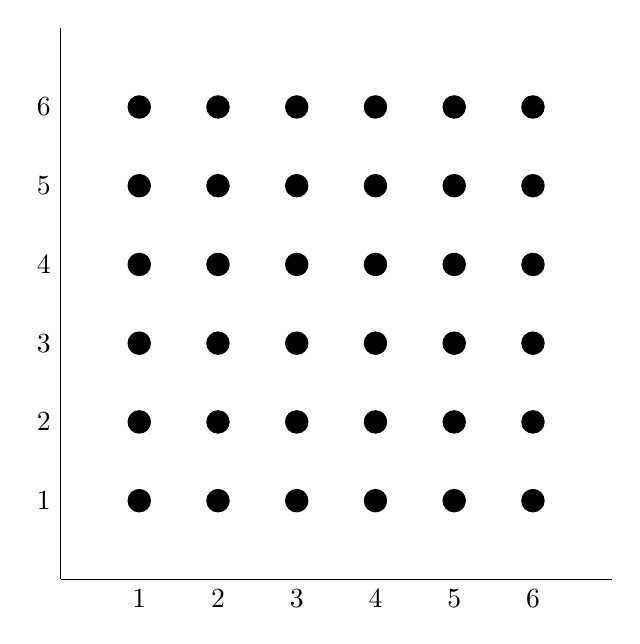
\begin{tikzpicture}[scale=1]
            \foreach \x in {1,...,6}
                {
                    \foreach \y in {1,...,6}
                        {
                            \node at (\x, \y)[circle,fill,inner sep=3pt]{};
                        }
                    \node[left] at (0, \x){$\x$};
                    \node[below] at (\x, 0){$\x$};
                }

            \draw (0.0, 0.0) -- (7.0, 0.0);
            \draw (0.0, 0.0) -- (0.0, 7.0);
        \end{tikzpicture}

        \small 图 1. 二维正方形格
    \end{center}

    \begin{center}
        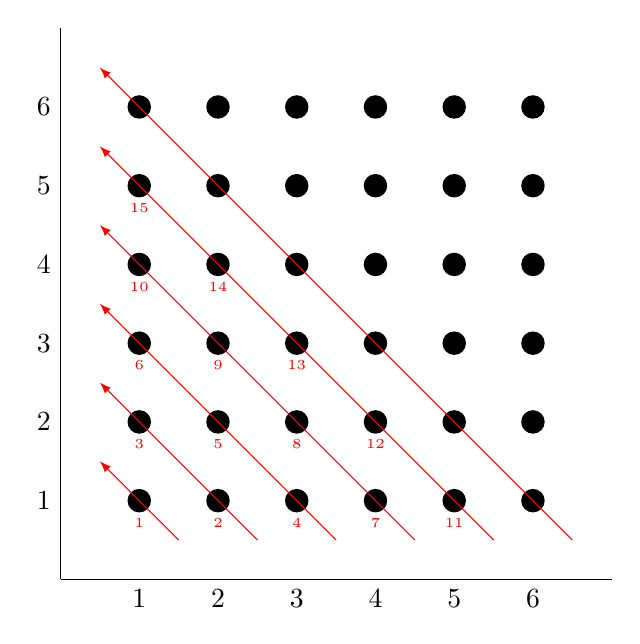
\begin{tikzpicture}[scale=1]
            \foreach \x in {1,...,6}
                {
                    \foreach \y in {1,...,6}
                        {
                            \node at (\x, \y)[circle,fill,inner sep=3pt]{};
                        }
                    \node[left] at (0, \x){$\x$};
                    \node[below] at (\x, 0){$\x$};
                    \draw[-latex, red] (\x+0.5, 0.5) -- (0.5, \x+0.5);
                }

            \draw (0.0, 0.0) -- (7.0, 0.0);
            \draw (0.0, 0.0) -- (0.0, 7.0);

            \foreach \y / \t in {1/1, 2/3, 3/6, 4/10, 5/15}
                {
                    \node[below,red] at (1, \y-0.1){\tiny$\t$};
                }
            \foreach \y / \t in {1/2, 2/5, 3/9, 4/14}
                {
                    \node[below,red] at (2, \y-0.1){\tiny$\t$};
                }
            \foreach \y / \t in {1/4, 2/8, 3/13}
                {
                    \node[below,red] at (3, \y-0.1){\tiny$\t$};
                }
            \foreach \y / \t in {1/7, 2/12}
                {
                    \node[below,red] at (4, \y-0.1){\tiny$\t$};
                }
            \node[below,red] at (5, 0.9){\tiny$11$};

        \end{tikzpicture}

        \small 图 2. 沿左上对角线遍历格中的点
    \end{center}
    \end{multicols}

    为了证明格上的无限多个顶点是\textbf{可数}无限的,我们可以描述一条路径,该路径遍历所有点(满射),且每个点只被遍历一次(单射),并用自然数进行索引(可数无限)。换句话说,我们可以通过一系列步骤遍历格中的所有点,从而定义出``第一个点''、``第二个点''等顺序。

    关键之处在于,格中沿左上方向的对角线都是\textbf{有限的}。例如,从点 $(5, 1)$ 开始,向左上方向沿对角线移动,会经过 $(4, 2), (3, 3), (2, 4), (1, 5)$,最终到达格的边界。无论从哪一行开始,沿左上方向移动都会到达边界。

    利用这一事实,我们可以根据 (a) 点所在的对角线,以及 (b) 点在该对角线上的位置,用自然数标记每个点。将从 $(1, 1)$ 开始的对角线作为第一条对角线,从 $(2, 1)$ 开始的对角线作为第二条对角线,依此类推。这样就得到如上图 2 的标注。

    可以看出,格中的每个点都恰好落在某条对角线上。此外,对角线的数量是可数无限的(由 $\mathbb{N}$ 索引),而每条对角线上只有\emph{有限}多个点。这意味着(我们将在下面进一步证明)所有对角线上的点构成的集合是可数无限集。

    你可以尝试通过定义一个函数来\emph{形式化}我们展示的标记方法。或者,也可以采用类似的方法,例如向右下方向移动,或交替反转对角线的方向……
\end{example}

\begin{example}[$\mathbb{Q}$ 是可数无限集]

    这个结果在处理无限集及其基数时,是直觉失灵的一个显著例子。想象一下,将 $\mathbb{Q}$ 的元素分布在数轴上,它们似乎无处不在!事实上,回顾练习 \ref{exc:exercises4.11.26},你证明了有理数是\textbf{稠密的},即在 $\mathbb{R}$ 中任意两个不同实数之间都存在一个有理数。此外,有理数集\emph{看起来}比整数集 $\mathbb{Z}$ 大得多:仅在 $0$ 和 $1$ 之间,就有无穷多个有理数!基于这些原因,你可能会认为 $\mathbb{Q}$ 是不可数无限集,但这一直觉是错误的。

    在本例中,我们将提供几个论证来证明 $\mathbb{Q}$ 是可数无限集,因为这个结论确实非常神奇且令人惊讶。

    \begin{enumerate}[label=(\arabic*)]
        \item \textbf{直观解释:}\\
              考虑以下将 $\mathbb{Q}$ 表示为集合并集的形式:
              \[\mathbb{Q} \;\text{``}=\text{''}\; \big(\text{``}\mathbb{N} \times \mathbb{N}\text{''}\big) \cup \big(\text{``}-(\mathbb{N} \times \mathbb{N})\text{''}\big) \cup \{0\}\]
              某种意义上,$\mathbb{N} \times \mathbb{N}$ 对应所有正有理数。为了理解这一点,考虑函数 $f : \mathbb{N} \times \mathbb{N} \to \mathbb{Q}_+$,定义为 $f(x, y) = \frac{x}{y}$。这个函数能生成所有正有理数(因此 $f$ 是满射),但由于 $\frac{4}{2}=\frac{2}{1}$,所以它不是单射。因为 $f$ 是满射,这至少表明 $|\mathbb{N} \times \mathbb{N}| \ge |\mathbb{Q}|$。由于 $\mathbb{N} \times \mathbb{N}$ 是可数无限集,而 $\mathbb{Q}$ 显然是无限集,这表明正有理数是可数无限集。\\

              负有理数集 $\mathbb{Q}_-$ 与正有理数集 $\mathbb{Q}_+$ 具有相同的基数。它们之间存在明确的双射关系:定义函数 $g : \mathbb{Q}_+ \to \mathbb{Q}_-$ 为 $\forall q \in \mathbb{Q}_+ \centerdot g(q) = -q$。\\

              这里唯一遗漏的是 $0 \in \mathbb{Q}$。两个可数无穷集的并集仍是可数无穷集(我们将在下面证明),再加上一个元素也不会改变这一点。因此,$\mathbb{Q}$ 是可数无限集。\\

              需要注意的是,上述论证有些``随意''。``等式''中的``引号''表示应将其视为启发性论证,而非严格证明。然而,确实有方法可以使此论证形式化。试着自己动手尝试一下吧!\\
        \item \textbf{列出 $\mathbb{Q}$ 中元素:}\\
              考虑编写一个计算机程序来列出所有正有理数。你会使用什么算法?只要保证程序``最终''能列出所有有理数,就证明了 $\mathbb{Q}$ 可以逐个枚举,因此它是可数无限集。(这也是为什么我们使用 $\mathbb{N}$ 作为典型的可数无限集:它的元素可以逐个枚举,我们可以数出它们。)\\

              一种编写程序的方法是采用前例中 $\mathbb{N} \times \mathbb{N}$ 的``格点路径''论证。但这次需要``跳过''已经打印过的有理数。\\

              具体来说,先打印 $(1, 1) \leftrightarrow 1$,然后是 $(2, 1) \leftrightarrow 2$,接着是 $(1, 2) \leftrightarrow \frac{1}{2}$,再是 $(3, 1) \leftrightarrow 3$,依此类推……\\

              注意,我们需要跳过 $(2, 2) \leftrightarrow 1$,因为 $1$ 已经打印过。如何判断某个数是否已经打印过?只需检查已打印的有理数列表,若要打印的数已存在则跳过,否则打印并继续。\\

              在枚举过程中,对于每个格点,我们只需检查\emph{有限}项——即已打印的\emph{有限多的}有理数集合。这意味着每一步打印会花费``稍长一点的时间'',但不会\emph{无限长}。因此,程序最终会列出每个有理数;无论你想到哪个有理数,我们都会在有限时间内到达它。\\
        \item \textbf{$\mathbb{Q}$ 至多是可数无限集:}\\
              这是 $\mathbb{Q}$ 是可数集的另一个论证。(如果觉得冗余,可以跳过。但我们认为从多个角度思考这一有趣结果是有益的!)\\

              请思考一下:我们可以先验地认为 $|\mathbb{Q}| \ge |\mathbb{N}|$,因为 $\mathbb{Q} \supseteq \mathbb{N}$。现在的问题是这两个基数是否相等。为了得出结论,我们需要找到:
              \begin{enumerate}[label=(\alph*)]
                  \item 从 $\mathbb{Q}$ 到某个可数集的单射;
                  \item 从某个可数集到 $\mathbb{Q}$ 的满射。\\
              \end{enumerate}

              我们将在后面证明 $\mathbb{Z} \times \mathbb{N}$ 是可数的(即任意两个可数无限集的笛卡尔积也是可数无限集)。定义函数 $f : \mathbb{Z} \times \mathbb{N} \to \mathbb{Q}$ 为:
              \[\forall (z, n) \in \mathbb{Z} \times \mathbb{N} \centerdot f(z, n) = \frac{z}{n}\]
              该函数是 $\mathbb{Q}$ 上的满射。尽管它不是单射(为什么?),但这不影响结论。它表明 $|\mathbb{Z} \times \mathbb{N}| = |\mathbb{Q}|$。一旦证明 $|\mathbb{Z} \times \mathbb{N}| = |\mathbb{N}|$,即可得出 $|\mathbb{N}| = |\mathbb{Q}|$。\\
        \item \textbf{Stern-Brocot 树:}\\
              $\mathbb{Q}$ 还有其他视觉表示方法,其中 \textbf{Stern-Brocot 树}尤其具有启发性。这一概念最早由法国钟表匠 Achille Brocot 提出,他在制作钟表时需要找到齿轮齿数的近似值。大约在同一时期($19$ 世纪 $50$ 年代和 $60$ 年代),德国数学家 Moritz Stern 也独立发展了这一思想。令人惊讶的是,一位非数学家竟能\emph{独立}提出如此迷人的概念来解决实际问题!\\

              (不必过于担心\emph{图}和\emph{树}等术语。我们不会深入讨论它们,这里只是简单介绍一下,以帮助理解 $\mathbb{Q}$ 的表示方法,并证明其为可数无穷集。)\\

              这棵树的\textbf{根节点}为 $1$(即图中最顶端的数字)。\textbf{父节点与子节点的关系}(即如何生成树的下一层节点)是通过连分数定义的(这里不详细解释其含义,而是描述构建过程)。\\

              通过这种构造方法,从根节点到任一节点的路径会产生一系列有理数,这些有理数逐渐逼近最终的节点。此外,序列中每个后续有理数的分母比前一个更大。这正是 Brocot 先生的动机:他需要确定两个齿轮的齿数比,使其接近特定值。通过沿树向下搜索,他可以找到更接近所需比率的近似值!是不是很酷?

              \begin{center}
                  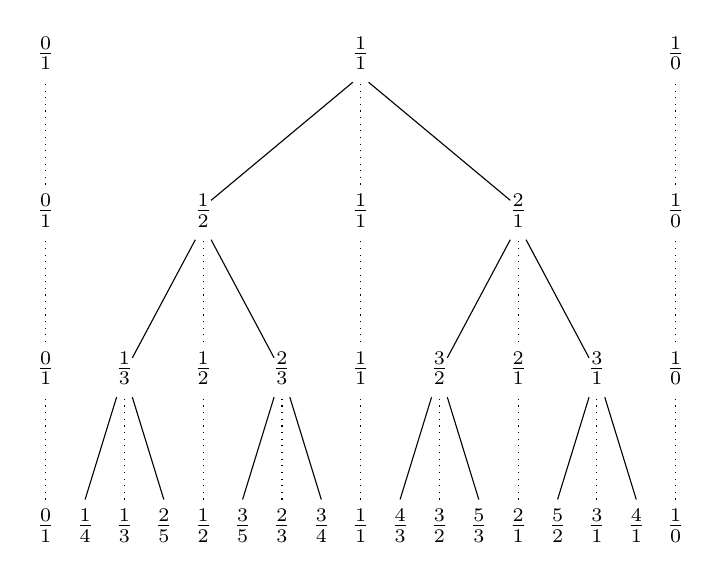
\begin{tikzpicture}[scale=1]
                      \edef \step {0.5};
                      \foreach \a / \b in {1/4, 1/3, 2/5, 1/2, 3/5, 2/3, 3/4}
                          {
                              \node[below] at (\step, 0){$\frac{\a}{\b}$};
                              \node[below] at (8-\step, 0){$\frac{\b}{\a}$};
                              \pgfmathparse{\step + 0.5};
                              \xdef \step{\pgfmathresult};
                          }

                      \edef \step {1.0};
                      \foreach \a / \b in {1/3, 1/2, 2/3}
                          {
                              \node[below] at (\step, 2){$\frac{\a}{\b}$};
                              \node[below] at (8-\step, 2){$\frac{\b}{\a}$};
                              \pgfmathparse{\step + 1.0};
                              \xdef \step{\pgfmathresult};
                          }

                      \node[below] at (2, 4){$\frac{1}{2}$};
                      \node[below] at (6, 4){$\frac{2}{1}$};

                      \foreach \y in {0,...,3}
                          {
                              \node[below] at (0, \y*2){$\frac{0}{1}$};
                              \node[below] at (4, \y*2){$\frac{1}{1}$};
                              \node[below] at (8, \y*2){$\frac{1}{0}$};
                          }

                      \edef \mx {0.1};
                      \edef \mya {0.2};
                      \edef \myb {0.7};
                      \foreach \y in {0,...,2}
                          {
                              \draw[dotted] (4, \y*2) -- (4, \y*2 + 2-\myb);
                          }

                      \foreach \x in {0,...,3}
                          {
                              \draw[dotted] (\x, 0.0) -- (\x, 2-\myb);
                              \draw[dotted] (8-\x, 0.0) -- (8-\x, 2-\myb);
                              \draw (\x*2+0.5, 0.0) -- (\x*2+1-\mx, 2-\myb);
                              \draw (\x*2+1.5, 0.0) -- (\x*2+1+\mx, 2-\myb);
                          }
                      \foreach \x in {0,...,1}
                          {
                              \draw[dotted] (\x*2, 2.0) -- (\x*2, 4-\myb);
                              \draw[dotted] (8-\x*2, 2.0) -- (8-\x*2, 4-\myb);
                              \draw (\x*4+1+\mx, 2.0-\mya) -- (\x*4+2-\mx, 4-\myb);
                              \draw (\x*4+3-\mx, 2.0-\mya) -- (\x*4+2+\mx, 4-\myb);
                          }
                      \foreach \x in {0}
                          {
                              \draw[dotted] (\x*8, 4.0) -- (\x*8, 6-\myb);
                              \draw[dotted] (8-\x*8, 4.0) -- (8-\x*8, 6-\myb);
                              \draw (\x*8+2+\mx, 4.0-\mya) -- (\x*8+4-\mx, 6-\myb);
                              \draw (\x*8+6-\mx, 4.0-\mya) -- (\x*8+4+\mx, 6-\myb);
                          }
                  \end{tikzpicture}
              \end{center}

              实际\emph{构建}这棵树时,需要计算\emph{中位数}。给定两个有理数 $\frac{a}{b}$ 和 $\frac{c}{d}$,它们的中位数定义为 $\frac{a+c}{b+d}$。(注意,这里的中位数是一种特殊对象,并非两个分数的加法!)\\

              树的每一层由上一层中相邻有理数对的所有中位数组成;我们不``计算''直接垂直的元素,它们仅用于辅助阅读和构建。此外,分数 $\frac{0}{1}$ 和 $\frac{1}{0}$(尽管 $\frac{1}{0}$ 未定义)包含在外侧列中,用于辅助生成每层最外侧的元素。\\

              (建议探索这棵树的性质并阅读更多\href{https://en.wikipedia.org/wiki/Stern%E2%80%93Brocot_tree}{相关内容}。这是一个非常有趣的数学对象!)\\

              这里不证明该树包含\emph{所有}有理数,但我们相信你能理解其合理性。此外,我们同样相信你能理解为什么树中所有节点的集合是\textbf{可数}无限集:每一层有有限个节点,而层数是可数无穷的。
    \end{enumerate}

\end{example}

\subsubsection*{定理}

现在我们知道,标准数集 $\mathbb{N}$、$\mathbb{Z}$ 和 $\mathbb{Q}$,以及 $\mathbb{N} \times \mathbb{N}$,都是可数无限集。接下来,通过一系列定理,我们将展示如何从这些已知集合出发,生成更多的可数无限集。

首先介绍一个有用的结论:若向一个可数无限集中``添加''有限多个元素,所得集合仍是可数无限集。

\begin{lemma}\label{lemma7.6.16}
    若 $A$ 为可数无限集,$B$ 为有限集且 $A \cap B = \varnothing$,则 $A \cup B$ 为可数无限集。
\end{lemma}

\begin{proof}
    留作练习 \ref{exc:exercises7.8.19}

    (\textbf{提示}:参考定理 \ref{theorem7.6.7} 的证明思路。)
\end{proof}

\begin{remark}
    注意:此引理中假设 $A \cap B = \varnothing$ 并非\emph{必要},但可简化证明。

    当 $A \cap B \ne \varnothing$ 时,可将已证结论应用于集合 $A - B$(可数无限集)与 $B - A$(有限集),得到可数无限集 $(A - B) \cup (B - A)$(因为二者互不相交)。再对集合 $(A - B) \cup (B - A)$ 与 $A \cap B$ 应用上述结论,从而得到可数无限集:
    \[A \cup B = (A - B) \cup (B - A) \cup (A \cap B)\]
\end{remark}

以下结论表明,该方法同样适用于 $A$ 和 $B$ 都是可数无限集的情况。

\begin{lemma}\label{lemma7.6.18}
    若 $A$ 和 $B$ 均为可数无限集,且 $A \cap B = \varnothing$,则 $A \cup B$ 为可数无限集。
\end{lemma}

\begin{proof}
    由于 $A$ 和 $B$ 均为可数无限集,故存在双射 $f : A \to \mathbb{N}$ 和 $g : B \to \mathbb{N}$。给定这些函数,我们需要构造一个双射 $h : A \cup B \to \mathbb{N}$。

    首先定义函数 $p : \mathbb{N} \to \mathbb{Z} - \mathbb{N}$ 为 $\forall n \in \mathbb{N} \centerdot p(n) = -n + 1$。

    这是一个双射,因为其反函数 $p^{-1} : \mathbb{Z} - \mathbb{N} \to \mathbb{N}$ 为 $p^{-1}(z) = -z + 1$。(读者可自行验证!)

    由于 $p$ 和 $g$ 都是双射,所以复合函数 $p \circ g : \mathbb{Z} - \mathbb{N}$ 也是双射。

    接下来定义分段函数 $q : A \cup B \to \mathbb{Z}$ 为
    \[\forall x \in A \cup B \centerdot q(x) = \begin{cases}
            f(x)    & \text{若}\; x \in A \\
            p(g(x)) & \text{若}\; x \in B
        \end{cases}\]
    由于 $A \cap B = \varnothing$,所以该函数是良定义的。此外,它也是一个双射,因为每一段函数都是双射。(读者可自行检验其合理性。练习 \ref{exc:exercises7.8.31} 给出了一般情况的证明。)

    综上,我们可以构造一个双射 $r : \mathbb{Z} \to \mathbb{N}$。(具体方法请参考示例 \ref{ex:example7.6.12}。)

    最后,定义函数 $h : A \cup B \to \mathbb{N}$ 为 $h = r \circ q$。由于 $r$ 和 $q$ 都是双射,它们的复合 $h$ 也是双射。这证明了 $|A \cup B| = |\mathbb{N}|$,即 $A \cup B$ 为可数无限集。
\end{proof}

接下来的推论表明,我们实际上不需要假设 $A \cap B = \varnothing$。这个假设仅是为了简化证明过程。我们鼓励你尝试证明这个推论。

\begin{corollary}\label{corollary7.6.19}
    若 $A$ 和 $B$ 均为可数无限集,则 $A \cup B$ 为可数无限集。
\end{corollary}

\begin{proof}
    留作练习 \ref{exc:exercises7.8.20}。

    (\textbf{提示}:将引理 \ref{lemma7.6.18} 应用于适当的集合上……)
\end{proof}

以上我们证明了几个关于集合\emph{并集}的结论。接下来,我们将证明关于\emph{笛卡尔积}的结论。

\begin{theorem}
    若 $A$ 和 $B$ 均为可数无限集,则 $A \times B$ 为可数无限集。
\end{theorem}

这个证明其实很简单,因为我们已经证明了关于 $\mathbb{N} \times \mathbb{N}$ 的结论:该集合是笛卡尔积,并且是可数无限集。在证明中,我们将展示如何利用 $\mathbb{N} \times \mathbb{N}$:

\begin{proof}
    假设 $A$ 和 $B$ 均为可数无限集,则存在双射 $ f : A \to \mathbb{N}$ 和 $g : B \to \mathbb{N}$。给定这样的函数。

    定义函数 $h : A \times B \to \mathbb{N} \times \mathbb{N}$ 为
    \[\forall (x, y) \in A \times B \centerdot h(x, y) = \big(f(x), g(y)\big)\]
    我们声称 $h$ 为双射。因为 $f, g$ 均可逆,定义函数 $H : \mathbb{N} \times \mathbb{N} \to A \times B$ 为
    \[\forall (k, \ell) \in \mathbb{N} \times \mathbb{N} \centerdot H(k, \ell) = \big(f^{-1}(k), g^{-1}(\ell)\big)\]
    我们声称 $H = h^{-1}$。因为
    \begin{align*}
        \forall (x, y) \in A \times B \centerdot (H \circ h)(x, y) & = H(h(x, y)) = H \big(f(x), g(y)\big)           \\
                                                                   & = \big(f^{-1}(f(x)), g^{-1}g((y))\big) = (x, y)
    \end{align*}
    且
    \begin{align*}
        \forall (k, \ell) \in \mathbb{N} \times \mathbb{N} \centerdot (h \circ H)(k, \ell) & = h(H(k, \ell)) = h\big(f^{-1}(k), g^{-1}(\ell)\big)  \\
                                                                                           & = \big(f(f^{-1}(k)), g(g^{-1}(\ell))\big) = (k, \ell)
    \end{align*}
    所以 $H \circ h = \id_{A \times B}$ 且 $h \circ H = \id_{\mathbb{N} \times \mathbb{N}}$。这表明 $H = h^{-1}$。

    因此,$h$ 为双射,故 $|A \times B| = |\mathbb{N} \times \mathbb{N}| = |\mathbb{N}|$。
\end{proof}

通过对前两个结论进行归纳,我们可以证明以下推论:

\begin{corollary}\label{corollary7.6.21}
    假设 $A_1, \dots , A_n$ 为可数集(其中 $n \in \mathbb{N}$,即我们有可数无限个集合),则 $A_1 \cup \dots \cup A_n$ 和 $A_1 \times \dots \times A_n$ 均为可数无限集。
\end{corollary}

\begin{proof}
    留作练习 \ref{exc:exercises7.8.22}。
\end{proof}

\subsubsection*{可数个可数集的并集为可数集}

你可能会好奇,当我们对\emph{可数无穷多}个集合(每个集合都是可数无限集)进行并集或笛卡尔积运算时,会发生什么情况。我们先来探讨并集的情形。这个结论非常基本且重要,我们甚至在章节标题中对其进行了强调!

\begin{theorem}\label{theorem7.6.22}
    对于每个 $n \in \mathbb{N}$,设 $A_n$ 为可数无限集,则集合
    \[A = \bigcup_{n \in \mathbb{N}} A_n = A_1 \cup A_2 \cup A_3 \cup \dots\]
    为可数无限集。
\end{theorem}

我们将证明集合\textbf{互不相交}的情况,其余细节留给你来完善。

\begin{proof}
    对于每个 $n \in \mathbb{N}$,设 $A_n$ 为可数无限集,且满足 $\forall i, j \in \mathbb{N} \centerdot i \ne j \implies A_i \cap A_j = \varnothing$。\\
    定义
    \[A = \bigcup_{n \in \mathbb{N}} A_n\]
    我们声称 $A$ 为可数无限集。

    由于每个 $A_n$ 都是可数无限集,故对每个 $n \in \mathbb{N}$,存在双射 $f_n : A_n \to \mathbb{N}$。这使我们可以根据 $f_n$ 对每个 $A_n$ 中的元素进行``编号''。同时,我们通过 $\mathbb{N}$ 对集合 $A_n$ 本身进行编号。本质上,我们为 $A$ 的元素赋予了一种对应于 $\mathbb{N} \times \mathbb{N}$ 的编号。下面正式定义这种对应关系。

    定义函数 $F : A \to \mathbb{N} \times \mathbb{N}$。给定任意 $x \in A$,我们知道 $\exists n \in \mathbb{N} \centerdot x \in A_n$ 且 $n$ 是\emph{唯一的}。(这是因为给定的集合互不相交)。令 $F(x) = \big(n, fn(x)\big)$。

    我们声称 $F$ 为双射。考虑函数 $G : \mathbb{N} \times \mathbb{N} \to A$,定义为
    \[\forall (a, b) \in \mathbb{N} \times \mathbb{N} \centerdot G(a, b) = f_a^{-1}(b)\]
    也就是说,$G$ 根据第一个坐标 $a$ 选取集合 $A_a$,然后通过函数 $f_a$ 确定 $A_a$ 中输出 $b \in \mathbb{N}$ 的元素。

    (请读者自行验证 $G = F^{-1}$。)

    由此可得 $|A| = |\mathbb{N} \times \mathbb{N}| = |\mathbb{N}|$,故 $A$ 是可数无限集。

    $A_n$ 可能相交的情况,留作练习 \ref{exc:exercises7.8.37}。
\end{proof}

\begin{corollary}\label{corollary7.6.23}
    对于每个 $n \in \mathbb{N}$,设 $A_n$ 为有限集,且这些集合互不相交。定义集合
    \[A = \bigcup_{n \in \mathbb{N}} A_n\]
    则 $A$ 为可数有限集。
\end{corollary}

\begin{proof}
    留作练习 \ref{exc:exercises7.8.36}。
\end{proof}

这个结论非常强大。让我们看两个应用示例。

\begin{example}[所有质数幂次的集合]
    还记得希尔伯特旅馆的讨论吗?在那个例子中,我们容纳了无穷多个会议,每个会议的人数也是无穷的。我们将客人安排到对应质数幂次的房间。对于每一个 $n \in \mathbb{N}$,定义 $p_n$ 为第 $n$ 个质数。则
    \[A_n = \{p_n^k \mid k \in \mathbb{N}\}\]
    为第 $n$ 个质数所有幂次的集合。上面的定理告诉我们
    \[\bigcup_{n \in \mathbb{N}} A_n = \{\text{质数的所有幂次}\}\]
    也是可数无限集。确实,这并不意外,因为该并集只是自然数的一个子集,而自然数本身是可数无限集!
\end{example}

\begin{example}[所有有限长二进制字符串的集合]\label{ex:example7.6.25}
    二进制字符串是由 \verb|0| 和 \verb|1| 组成的有序序列。\textbf{有限长二进制字符串}是指长度有限的二进制字符串。

    例如,以下都是有限长二进制字符串:
    \[0, \quad 1, \quad 101010, \quad 10000000000000000001 \]

    对于每个 $n \in \mathbb{N}$,定义 $F_n$ 为所有长度为 $n$ 的二进制字符串的集合。例如
    \begin{align*}
        F_1 & = \{ 0 , 1 \}                                         \\
        F_2 & = \{ 00 , 01 , 10 , 11 \}                             \\
        F_3 & = \{ 000 , 001 , 010 , 100 , 011 , 101 , 110 , 111 \}
    \end{align*}
    依此类推。(注意 $|F_n| = 2^n$,读者可以尝试证明这一点。)则所有有限长二进制字符串的集合定义为
    \[F = \bigcup_{n \in \mathbb{N}} F_n\]

    $F$ 的每个元素都属于某个 $F_n$,这意味着每个元素都是有限长二进制字符串。这个长度可能非常大,但它是有限的。(这说明了``任意大(但有限)''和``无限''之间的区别。)

    这个例子的重点是,根据上面的定理,$F$ 是可数的!(实际上,这可以从紧随其后的推论得出。)相比之下,所有\emph{无限长}二进制字符串的集合 $S$ 是不可数的 —— 我们很快会证明这一点。我们将经常使用这些二进制字符串集合作为例子!
\end{example}

\subsubsection*{取``极限''}

我们已经证明,如果 $A$ 和 $B$ 是可数无限集,那么 $A \cup B$ 和 $A \times B$ 也是可数无限集。我们还建议通过归纳法(对并集或乘积中的集合数量进行归纳)来证明,对于任意 $n \in \mathbb{N}$,
\[A_1 \cup A_2 \cup \dots \cup A_n = \bigcup_{i \in [n]} A_i \quad \text{和} \quad \prod_{i \in [n]} A_i = A_1 \times A_2 \times \dots \times A_n\] 
也是可数无限集。

这些结论是否为我们提供了某些关于
\[A_1 \cup A_2 \cup A_3 \cup \dots = \bigcup_{k \in \mathbb{N}} A_k \quad \text{和} \quad A_1 \times A_2 \times A_3 \times \dots = \prod_{k \in \mathbb{N}} A_k\]
的信息?也就是说,当我们尝试从\emph{有限}数量的并集或乘积(任意大但仍然有限)过渡到\emph{无限}数量的并集或乘积时,会发生什么?我们能得出必要的结论吗?我们能找到反例吗?

主要思想是,``取极限''确实会创建某些数学对象,但我们不能预先假设这个对象具有与定义它的序列中所有对象\emph{完全相同的属性}。

考虑有限集 $[n]$,对于每个 $n$,$[n]$ 都是有限的,但``取极限''后我们得到的 $\mathbb{N}$ 是无限的。因此,我们确实得到了一个对象(另一个集合),但它不一定具有相同的属性。

上述重要定理表明,在\emph{并集}中取极限肯定会保留可数性。正如我们将在下一节中看到的那样,\emph{乘积}肯定\textbf{不会}保留可数性。(实际上,即使是无限个有限集的乘积也是不可数的。真是令人惊讶!)

在微积分中也有类似的概念。我们原本承诺不使用微积分,但这些思想之间有如此自然的关系,因此我们不得不提及一个简单的例子。如果你不理解也没关系;如果你理解了,试着记住这个联系,并思考它如何从根本上改变了你在微积分中学到的一切。

考虑如下\emph{极限}:
\[\lim_{x \to \infty} \frac{1}{x} = 0\]
这个极限在何种意义上\textbf{等于} $0$?为什么身为数学家的我们会选择用这种方式\emph{定义}极限?形式上,这个极限是有意义的,因为它符合极限的量化定义。设 $P$ 为正实数集,极限的定义(应用于这个例子)为
\[\forall \varepsilon \in P \centerdot \exists M \in \mathbb{N} \centerdot \forall n \in \mathbb{N} \centerdot \big(n > M \implies \big|\frac{1}{x}\big| < \varepsilon \big)\]
也就是说,对于任意小的正阈值 $\varepsilon > 0$,我们都可以找到一个特定的截止点(一个依赖于 $\varepsilon$ 的自然数 $M$),使得在 $M$ \emph{之后}的每一个点,函数 $\frac{1}{x}$ 的值都在极限点 $0$ 的 $\varepsilon$ 范围内。

请注意,这与 ``$\frac{1}{\infty} = 0$'' 这样的说法\emph{完全不同}。事实并非如此。实际上,我们从未真正``代入''极限的终点来进行计算。极限是通过量化定义的,也就是说,我们讨论的是在\emph{任意大}值下发生的情况,而不是在\emph{无限大}值下发生的情况。
